% Template for PLoS
% Version 3.4 January 2017
%
% % % % % % % % % % % % % % % % % % % % % %
%
% -- IMPORTANT NOTE
%
% This template contains comments intended 
% to minimize problems and delays during our production 
% process. Please follow the template instructions
% whenever possible.
%
% % % % % % % % % % % % % % % % % % % % % % % 
%
% Once your paper is accepted for publication, 
% PLEASE REMOVE ALL TRACKED CHANGES in this file 
% and leave only the final text of your manuscript. 
% PLOS recommends the use of latexdiff to track changes during review, as this will help to maintain a clean tex file.
% Visit https://www.ctan.org/pkg/latexdiff?lang=en for info or contact us at latex@plos.org.
%
%
% There are no restrictions on package use within the LaTeX files except that 
% no packages listed in the template may be deleted.
%
% Please do not include colors or graphics in the text.
%
% The manuscript LaTeX source should be contained within a single file (do not use \input, \externaldocument, or similar commands).
%
% % % % % % % % % % % % % % % % % % % % % % %
%
% -- FIGURES AND TABLES
%
% Please include tables/figure captions directly after the paragraph where they are first cited in the text.
%
% DO NOT INCLUDE GRAPHICS IN YOUR MANUSCRIPT
% - Figures should be uploaded separately from your manuscript file. 
% - Figures generated using LaTeX should be extracted and removed from the PDF before submission. 
% - Figures containing multiple panels/subfigures must be combined into one image file before submission.
% For figure citations, please use "Fig" instead of "Figure".
% See http://journals.plos.org/plosone/s/figures for PLOS figure guidelines.
%
% Tables should be cell-based and may not contain:
% - spacing/line breaks within cells to alter layout or alignment
% - do not nest tabular environments (no tabular environments within tabular environments)
% - no graphics or colored text (cell background color/shading OK)
% See http://journals.plos.org/plosone/s/tables for table guidelines.
%
% For tables that exceed the width of the text column, use the adjustwidth environment as illustrated in the example table in text below.
%
% % % % % % % % % % % % % % % % % % % % % % % %
%
% -- EQUATIONS, MATH SYMBOLS, SUBSCRIPTS, AND SUPERSCRIPTS
%
% IMPORTANT
% Below are a few tips to help format your equations and other special characters according to our specifications. For more tips to help reduce the possibility of formatting errors during conversion, please see our LaTeX guidelines at http://journals.plos.org/plosone/s/latex
%
% For inline equations, please be sure to include all portions of an equation in the math environment.  For example, x$^2$ is incorrect; this should be formatted as $x^2$ (or $\mathrm{x}^2$ if the romanized font is desired).
%
% Do not include text that is not math in the math environment. For example, CO2 should be written as CO\textsubscript{2} instead of CO$_2$.
%
% Please add line breaks to long display equations when possible in order to fit size of the column. 
%
% For inline equations, please do not include punctuation (commas, etc) within the math environment unless this is part of the equation.
%
% When adding superscript or subscripts outside of brackets/braces, please group using {}.  For example, change "[U(D,E,\gamma)]^2" to "{[U(D,E,\gamma)]}^2". 
%
% Do not use \cal for caligraphic font.  Instead, use \mathcal{}
%
% % % % % % % % % % % % % % % % % % % % % % % % 
%
% Please contact latex@plos.org with any questions.
%
% % % % % % % % % % % % % % % % % % % % % % % %

\documentclass[10pt,letterpaper]{article}
\usepackage[top=0.85in,left=2.75in,footskip=0.75in]{geometry}

% amsmath and amssymb packages, useful for mathematical formulas and symbols
\usepackage{amsmath,amssymb}

% Use adjustwidth environment to exceed column width (see example table in text)
\usepackage{changepage}

% Use Unicode characters when possible
\usepackage[utf8x]{inputenc}

% textcomp package and marvosym package for additional characters
\usepackage{textcomp,marvosym}

% cite package, to clean up citations in the main text. Do not remove.
\usepackage{cite}


% Use nameref to cite supporting information files (see Supporting Information section for more info)
\usepackage{nameref,hyperref}

% line numbers
\usepackage[right]{lineno}

% ligatures disabled
\usepackage{microtype}
\DisableLigatures[f]{encoding = *, family = * }

% color can be used to apply background shading to table cells only
\usepackage[table]{xcolor}

% array package and thick rules for tables
\usepackage{array}

% create "+" rule type for thick vertical lines
\newcolumntype{+}{!{\vrule width 2pt}}

% create \thickcline for thick horizontal lines of variable length
\newlength\savedwidth
\newcommand\thickcline[1]{%
  \noalign{\global\savedwidth\arrayrulewidth\global\arrayrulewidth 2pt}%
  \cline{#1}%
  \noalign{\vskip\arrayrulewidth}%
  \noalign{\global\arrayrulewidth\savedwidth}%
}

% \thickhline command for thick horizontal lines that span the table
\newcommand\thickhline{\noalign{\global\savedwidth\arrayrulewidth\global\arrayrulewidth 2pt}%
\hline
\noalign{\global\arrayrulewidth\savedwidth}}


% Remove comment for double spacing
%\usepackage{setspace} 
%\doublespacing

% Text layout
\raggedright
\setlength{\parindent}{0.5cm}
\textwidth 5.25in 
\textheight 8.75in

% Bold the 'Figure #' in the caption and separate it from the title/caption with a period
% Captions will be left justified
\usepackage[aboveskip=1pt,labelfont=bf,labelsep=period,justification=raggedright,singlelinecheck=off]{caption}
\renewcommand{\figurename}{Fig}

% Use the PLoS provided BiBTeX style
\bibliographystyle{plos2015}

% Remove brackets from numbering in List of References
\makeatletter
\renewcommand{\@biblabel}[1]{\quad#1.}
\makeatother

% Leave date blank
\date{}

% Header and Footer with logo
\usepackage{lastpage,fancyhdr,graphicx}
\usepackage{epstopdf}
\pagestyle{myheadings}
\pagestyle{fancy}
\fancyhf{}
\setlength{\headheight}{27.023pt}
\lhead{\includegraphics[width=2.0in]{PLOS-submission.eps}}
\rfoot{\thepage/\pageref{LastPage}}
\renewcommand{\footrule}{\hrule height 2pt \vspace{2mm}}
\fancyheadoffset[L]{2.25in}
\fancyfootoffset[L]{2.25in}
\lfoot{\sf PLOS}

%% Include all macros below

\newcommand{\lorem}{{\bf LOREM}}
\newcommand{\ipsum}{{\bf IPSUM}}

%% END MACROS SECTION


\begin{document}
\vspace*{0.2in}

% Title must be 250 characters or less.
\begin{flushleft}
{\Large
\textbf\newline{Data Reconstruction Using Iteratively Reweighted L1-Principal Component Analysis for an Electronic Nose System} % Please use "sentence case" for title and headings (capitalize only the first word in a title (or heading), the first word in a subtitle (or subheading), and any proper nouns).
}
\newline
% Insert author names, affiliations and corresponding author email (do not include titles, positions, or degrees).
\\
Hong-Min Jeon\textsuperscript{1},
Je-Yeol Lee\textsuperscript{2},
Gu-Min Jeong\textsuperscript{3},
Sang-Il Choi\textsuperscript{2,*}
\\
\bigskip
\bf{1} Korean Research Institute of Bioscience and Biotechnology,
125 Gwahak-ro, Yuseong-gu, Daejeon 306-809, Korea.

\bf{2} Department of Computer Science and Engineering,
Dankook University, 152, Jukjeon-ro, Suji-gu, Yongin-si, Gyeonggi-do, 16890, Korea.

\bf{3} Electrical Engineering,
Kookmin University, 861-1, Jeongneung-dong, Seongbuk-gu, Seoul 02707, Korea.
\\
\bigskip

* choisi@dankook.ac.kr

\end{flushleft}
% Please keep the abstract below 300 words
\section*{Abstract}

We propose a method to reconstruct damaged data based on statistical learning during data acquisition. In the process of measuring the data using a sensor, the damage of the data caused by the defect of the sensor or the environmental factor greatly degrades the performance of data classification. Instead of the traditional PCA based on L2-norm, the PCA features were extracted based on L1-norm and updated by iteratively reweighted fitting using the generalized objective function to obtain robust features for the outlier data. The damaged data samples were reconstructed using weighted linear combination using these features and the projection vectors of L1-norm based PCA. The experimental results on various types of volatile organic compounds (VOCs) data show that the proposed method can be used to reconstruct the damaged data to the original form of the undamaged data and to prevent degradation of classification performance due to data corruption through data reconstruction. 

% Use "Eq" instead of "Equation" for equation citations.
\section*{Introduction}
The human olfactory sense is easily fatigued and cannot sustain smell; it also has a limitation whereby it cannot always precisely distinguish between similar smells. 
In contrast, an electronic nose system can continuously collect gas data and easily distinguish gas types, which is an advantage in various fields in which the human nose cannot be utilized \cite{berna2009bio,fonollosa2012quality}.

The electronic nose system that classifies the types of gas can be roughly divided into a sensor part that measures gas data and a computing system that extracts the features of the gas from the measured data and identifies the type of gas through the classifier \cite{ampuero2003electronic,gardner1994brief}. 
Sensors commonly used in electronic nose systems are electrochemical sensors such as a metal-oxide sensor \cite{barsan2007metal}, tin-oxide sensor \cite{watson1984tin}, and piezoelectric sensor such as a carbon-black senor \cite{kim2005portable} or a conducting organic sensor \cite{janata2003conducting}.

The computing system consists of three steps: a preprocessing step involving converting the measured data into a form suitable for feature extraction, a step involving extracting features for gas classification, and a step involving a classifier for identifying the type of gas with the extracted features. 
The features for gas classification can be extracted based on various statistical methodologies widely used in the field of pattern recognition \cite{belhumeur1997eigenfaces,fukunaga2013introduction,wang2007reconstruction}. 
Various methods based on the linear discriminant analysis (LDA) \cite{belhumeur1997eigenfaces,martinez2001pca,kim2007discriminant} or the principal component analysis (PCA) \cite{fukunaga2013introduction,turk1991eigenfaces,vergara2012chemical} can be used for efficient classification of high-dimensional data such as electronic nose data.

In most studies on feature extraction, it is assumed that the used data has no defect, so that if the data is partially lost or damaged, the intended performance cannot be obtained. 
However, in the case of the electronic nose system, since the system operating environment in the practical field is often poor, it may be difficult to collect high-quality data due to problems such as power supply or sensor defect. 
In this case, the classification performance of the probe data may be significantly degraded as it differs from the data used as the training data of the feature extraction. 

To solve this problem, statistical analysis methods can be used to restore corrupted data and the reconstructed data can then be used for classification. 
In \cite{wang2007reconstruction}, a conventional PCA based on L2-norm was used for data reconstruction. 
However, the L2-norm based PCA finds feature values to minimize the squared error between the sample and the reconstructed sample, which can excessively increase the sensitivity of the outliers \cite{kwak2008principal}. 
Also, since the PCA features are values obtained from a linear transformation of the data samples by the projection vectors, 
if noise or defects occur in the training data, distortion occurs in the projection vectors, rendering it difficult to obtain good features.

In this paper, we propose a method to reconstruct a data sample, some values of which are lost due to sensor instability in the electronic nose system. 
First, by using L1-norm maximization-based PCA (L1-PCA) \cite{kwak2008principal}, projection vectors less affected by outlier samples are obtained and the initial features are obtained through a linear transformation of data samples using projection vectors. 
Then, by repeatedly updating the initial feature values to satisfy the generalized objective function for the errors between the reconstructed sample and the original sample \cite{zuo2006robust}, better features for use in data reconstruction were obtained. 
The gas data samples reconstructed using the updated new features are classified through the discriminant feature extraction process and the classifier.

For the reconstruction experiment of lost data, we used data measurement using the carbon-black sensors for 8 types of gas, and we partially lost values of the data randomly\cite{yang2005matched}. 
We then evaluated the reconstruction performance by measuring the root mean squared (RMS) error of the reconstructed result using the proposed method and the lossless data. 
In addition, we confirmed the way in which the proposed reconstruction process can improve the gas classification performance by comparing the classification rates before and after reconstruction.

This paper is structured as follows. 
In the next section, we present the data reconstruction method using iteratively reweighted L1-principal component analysis. 
Then, we design the electronic nose system using the proposed data reconstruction method. 
Finally, the experimental results on data reconstruction and gas classification are described and the conclusion follows.

\section*{Data Reconstruction Using Iteratively Reweighted L1-Principal Component Analysis}
\subsection*{Iteratively Reweighted L1-PCA}

% For figure citations, please use "Fig" instead of "Figure".

When dealing with high-dimensional data such as electronic nose data, we can simplify the problem for effective analysis by using the dimension reduction method. 
PCA, which is a multi-variate analysis method based on statistical methodology, is one of the most popular methods for this purpose. 

\begin{figure}[t]
	\centering
    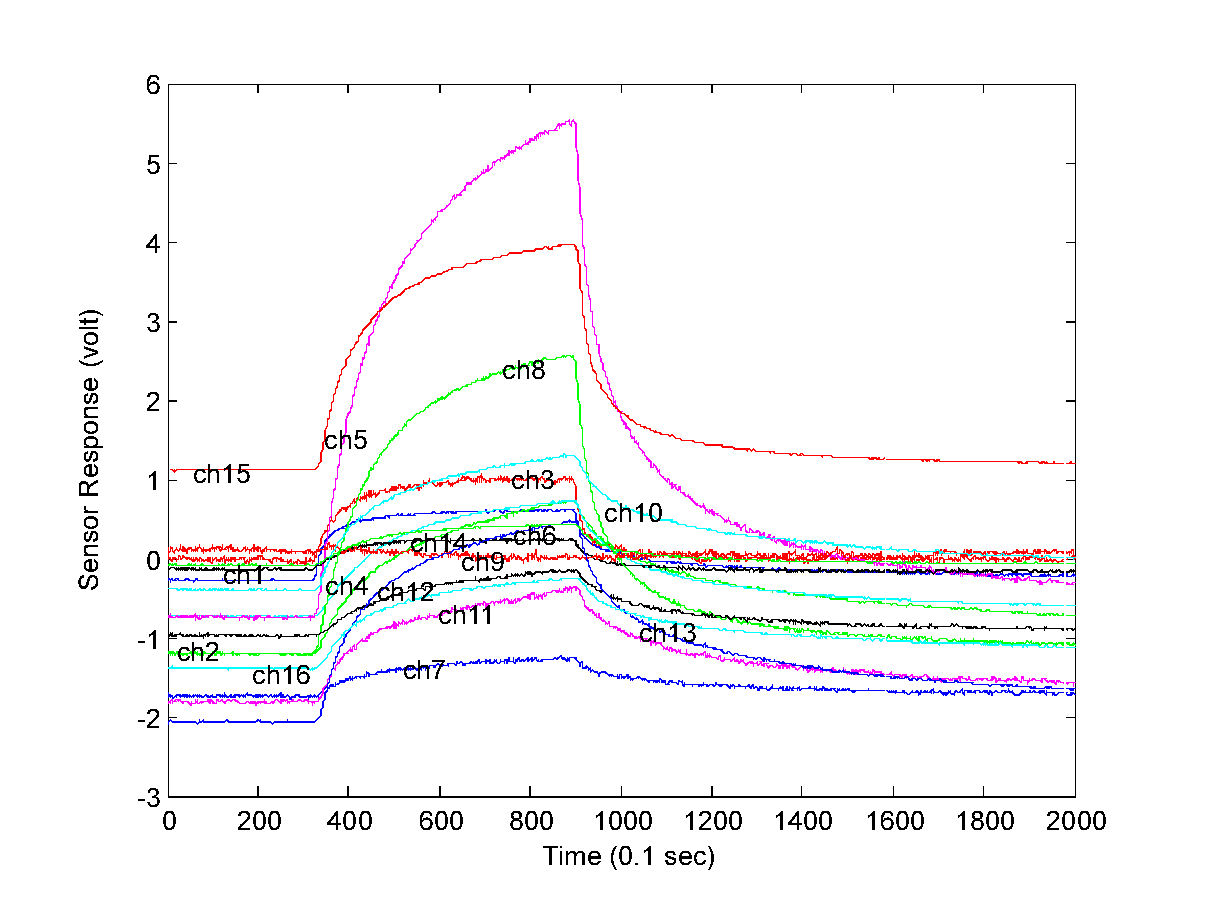
\includegraphics[width=0.8\textwidth]{fig1.eps}
    \caption{\bf{Typical time-response of 16 channel sensor array with respect to inflow of ethanol vapor.} \label{null Fig. 1}}
\end{figure}


Let us consider a data set consisting of $N$ samples. 
Each sample can be represented by a point $\textbf{x}_{k}=[x_{k1},..,x_{kn}]^T$ in the $n$-dimensional vector space. 
This space is called an input space, and each component of $\textbf{x}_{k}$ is called a primitive variable. 
In the conventional PCA, we find the projection vectors $\textbf{w}_{l}=[w_{l1},..,w_{ln}]^T$, $l = 1, ..., m$ that satisfy the following objective function based on L2-norm \cite{duda1973pattern}.

\begin{eqnarray}
\label{eq:IEEESensors3}
	{J_m} = \sum\limits_{k=1}^{N}||\left(\mu+\sum\limits_{l=1}^{m}{y}_{kl}\textbf{w}_l\right)-\textbf{x}_k||^2
\end{eqnarray}

Here, $\mu$ is the sample mean $\mu=\frac{1}{N}\sum\limits_{k = 1}^{N} {\textbf{x}_k}$ and ${y}_{kl}$s are principal components (PCA features corresponding to $\textbf{w}_{kl}$s). 

The global minimum of $J_m$ can be obtained by using the singular value decomposition (SVD) \cite{golub1970singular} to find $W$ that satisfies the following object function. 

\begin{eqnarray}
\label{eq:IEEESensors4}
	W\left(=[\textbf{w}_1,\textbf{w}_2,..,\textbf{w}_m]\right)=\textrm{arg} \underset{W}{\textrm{max}}||W^{T}S_{T}W||
\end{eqnarray}
Here, ${S}_{T}$ is a total scatter matrix and is defined as $S_T = \sum\limits_{k=1}^{N}(\textbf{x}_k-\mu)(\textbf{x}_k-\mu)^T$.

  
However, since the conventional PCA constructs a feature space that maximizes the dispersion of the samples based on the L2-norm, when an outlier data sample is present, the sample tends to have an excessive influence on the process of obtaining the projection vector. 
Therefore, we use L1-PCA \cite{kwak2008principal} based on L1-norm, which is more robust to outlier data than L2-norm for data reconstruction. 
In order to prevent distortion of the equidistance surface by the rotation of L1-norm, L1-PCA finds a projection vector that maximizes the L1 dispersion using L1-norm in the feature space by using the following objective function. 
\begin{eqnarray}
\label{eq:PAMI5}
	W^* = \textrm{arg} \underset{W}{\textrm{max}}\sum\limits_{k=1}^{N}\sum\limits_{l=1}^{m}\begin{vmatrix}\sum\limits_{i=1}^{n}w_{li}x_{ki}\end{vmatrix} \nonumber\\ \textrm{subject to } W^TW = I \in R^{m \times m}
\end{eqnarray}  

The optimal $l$-th projection vector, $\textbf{w}_l$, satisfying the objective function in (\ref{eq:PAMI5}) is changed according to the number of projection vectors ($m$) to be obtained and it is very difficult to obtain the global solution for (\ref{eq:PAMI5}) when $m > 1$. 
In order to avoid this problem, as in \cite{kwak2008principal}, we also obtain $\textbf{w}^{*}$ by using the following objective function when $m = 1$.
\begin{eqnarray}
\label{eq:PAMI6}
	\textbf{w}^* = \textrm{arg} \underset{W}{\textrm{max}}\sum\limits_{k=1}^{N}|\textbf{w}^{T}\textbf{x}_k| \textrm{ subject to }||\textbf{w}||_2 = 1
\end{eqnarray}
Then, we find an approximate solution ($W_{L1} = [\textbf{w}_{1}, \textbf{w}_{2},..,\textbf{w}_{m}]$) to (\ref{eq:PAMI5}) by using the greedy search method \cite{kwak2008principal}.

\begin{figure}[t]
	\centering
    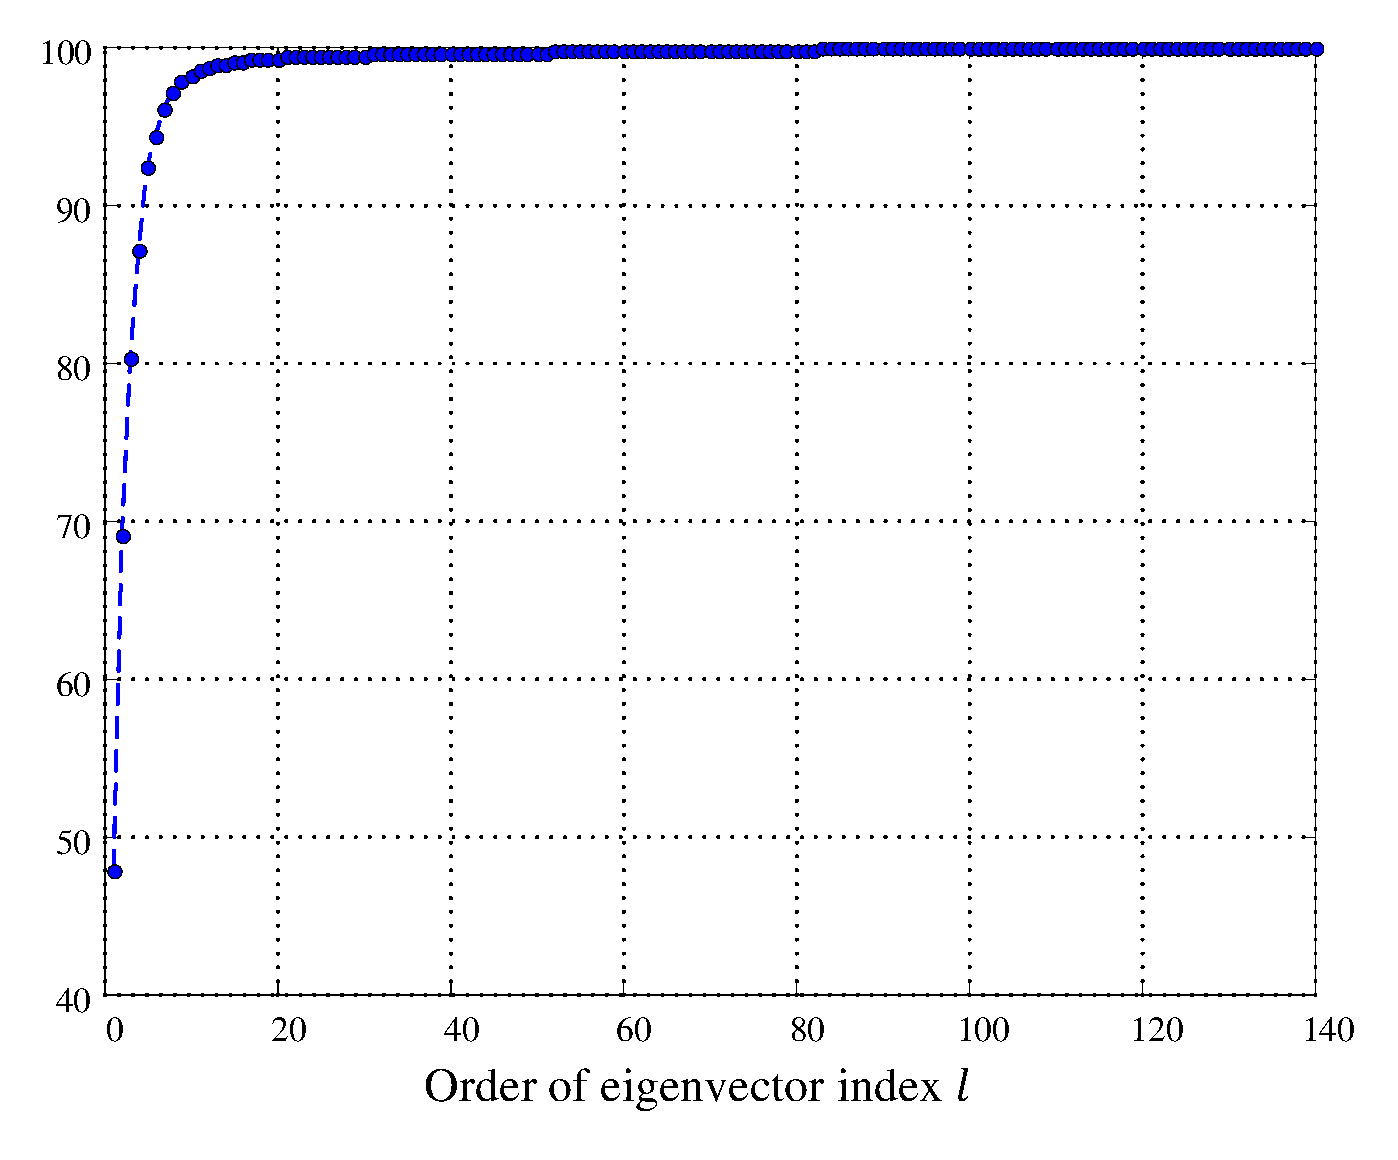
\includegraphics[width=0.8\textwidth]{eigenvector.eps}
    \caption{\bf{Cumulative sum percentage of eigenvalues after sorting the eigenvalues of the scatter matrix of e-nose data samples in descending order.} \label{null Fig. 2}}
\end{figure}
By using $W_{L1}$, the feature vector for the data sample is obtained through the following linear transformation.
\begin{eqnarray}
\label{eq:sic5}
	\textbf{y}_k = W_{L1}^T\left(\textbf{x}_k-\mu\right)
\end{eqnarray}

The features are then updated through the iteratively reweighted fitting (IRF) process \cite{zuo2006robust} to improve the effect of data reconstruction. 
To achieve this, a generalized objective function containing nonlinear mapping is defined as (\ref{eq:sic6}) and the projection vector is repeatedly weighted using the iteratively reweighted least squares (IRLS) \cite{ha2005integrated}.
\begin{eqnarray}
\label{eq:sic6}
	J(\textbf{y}) &=& \sum\limits_{i=1}^{n}G\left(\left(x_i-W_{i}\textbf{y}\right)^2\right)\nonumber\\ \mathrm G(z) &=& \log\frac{1}{1+\exp\left(-\beta\left(z-\eta\right)\right)}  
\end{eqnarray}
In (\ref{eq:sic6}), $\beta$ and $\eta$ (which are tuning parameters) are the inverse temperature and saturation value, respectively, and $W_i$ denotes the $i$-th row vector of $W_{L1}$. 

The process of minimizing the objective function in (\ref{eq:sic6}) can be divided into a weight calculation step and a least squares step \cite{zuo2006robust}. 
In the weighting step at each ($t$-th) iteration, a weight vector $\boldsymbol{\omega}^{\left(t\right)}=\left[{\omega}_{1}^{\left(t\right)},{\omega}_{2}^{\left(t\right)},..,{\omega}_{n}^{\left(t\right)}\right]^{T}$ is defined for a feature vector $\textbf{y}^{(t)}$, and its values are calculated as follows \cite{zuo2006robust}. 



\begin{eqnarray}
\label{eq:sic8}
	\mathrm \mathbf{\omega}_i^{\left(t\right)} = \frac{\exp\left(-\beta\left(z_i^{\left(t\right)}-\eta\right)\right)}{1+\exp\left(-\beta\left(z_i^{\left(t\right)}-\eta \right)\right)}
\end{eqnarray}

\begin{eqnarray}
\label{eq:sic7}
	\mathrm \mathit{z_i^{\left(t\right)}} = \left(x_i-W_{i}\mathbf{y}^{\left(t\right)}\right)^2
\end{eqnarray}

In the least squares step at the $(t+1)$-th iteration, the feature vector $\textbf{y}^{(t+1)}$ is updated with the weight vector $\boldsymbol{\omega}^{(t)}$ calculated in the weight step as follows.



\begin{eqnarray}
\label{eq:sic9}
	\textbf{y}^{(t+1)} = (\sum\limits_{i=1}^{n}{\omega}_i^{(t)}{W_i^T}{W_i})^{-1}\sum\limits_{i=1}^{n}{\omega}_i^{(t)}W_i^{T}x_i
\end{eqnarray}


In this manner, while repeating the weighting step and the least square step, the feature vector $(\textbf{y}^{(t)})$ updating is repeated until the convergence or termination condition $(t=t_{max})$ is satisfied.
\begin{figure}[t]
	\centering
    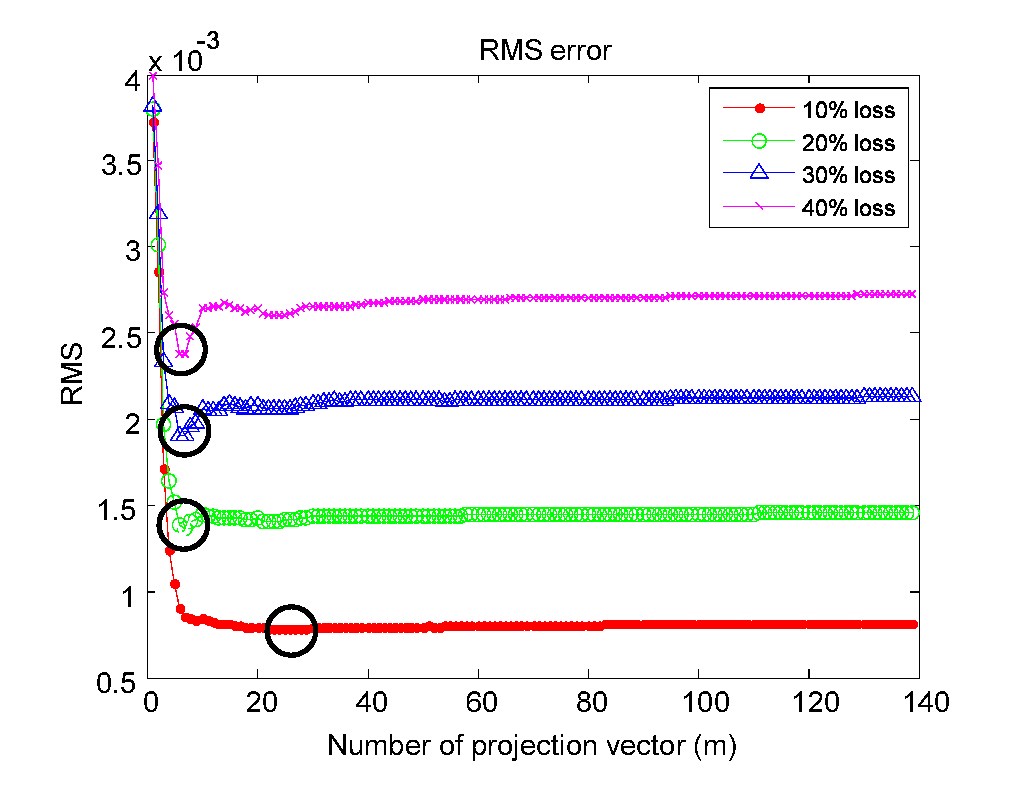
\includegraphics[width=1\textwidth]{fig3_1.eps}
    \caption{\bf{Observations of RMS errors for different numbers of projections vectors.}\label{Fig. 3}}
\end{figure}

\subsection*{Reconstruction of Distorted Data}
Fig. \ref{null Fig. 1} shows typical time-responses of a 16 channel sensor array for ethanol vapor. In the case of sensor data, data measurement may be partially lost or damaged depending on the installation environment and electrical environmental conditions. 
The lost or damaged data can be reconstructed using the projection vectors of the L1-PCA and the updated new L1-PCA features, which can be accomplished by simple matrix operations. 

As shown in (\ref{eq:PAMI5}), the projection vectors obtained through L1-PCA are orthogonal to each other; hence, $\textbf{x}_k$ is approximated as a linear combination of the basis $\textbf{w}_{l}$s that constitutes a feature space as follows.

\begin{eqnarray}
\label{eq:sic10}
	\textbf{x}_k \mathrm{=} W_{L1}\textbf{y}_{k}+\mu
\end{eqnarray}


The reconstructed data $\textbf{x}^{re}$ for the damaged data sample $\textbf{x}^{dmg}$ can be obtained by using \textit{m} projection vectors with high data representation power and the feature vector $\textbf{y}^{(t)}=[y_{1}^{(t)},y_{2}^{(t)},..,y_{m}^{(t)}]^{T}$ updated through the IRF as follows.

\begin{eqnarray}
\label{eq:sic11}
	\mathbf{y}_k &=& W_{L1}^T(\textbf{x}^{dmg}-\mu) \underset{IRF}{\longrightarrow} \textbf{y}_{k}^{(t)} \nonumber\\\textbf{x}^{re}_{k}&=&W_{L1}\mathbf{y}_{k}^{(t)}+\mu
\end{eqnarray} 



Fig. \ref{null Fig. 2} shows a graph plotting the cumulative sum percentage of eigenvalues after sorting the eigenvalues of the scatter matrix of electronic nose data samples in descending order. 
In Fig. 2, the magnitude of the eigenvalue $\lambda_l$ decreases sharply at the beginning with an increasing index $l$, which means that most of the eigenvalues are concentrated in a few major eigenvectors. 
The eigenvalue of the projection vector refers to the variance of the data samples in the feature space. 
However, the estimated eigenvalue $\lambda_l$ from the training samples somewhat differs from the true variance of the projected vector, due to the limited number of training samples. 
In particular, eigenvectors with small eigenvalues are sensitive to noise \cite{martinez1998ar}. 
Therefore, in this paper, we only use eigenvectors with large eigenvalues instead of using whole eigenvectors in the data reconstruction process.


\begin{figure}[h]
	\centering
    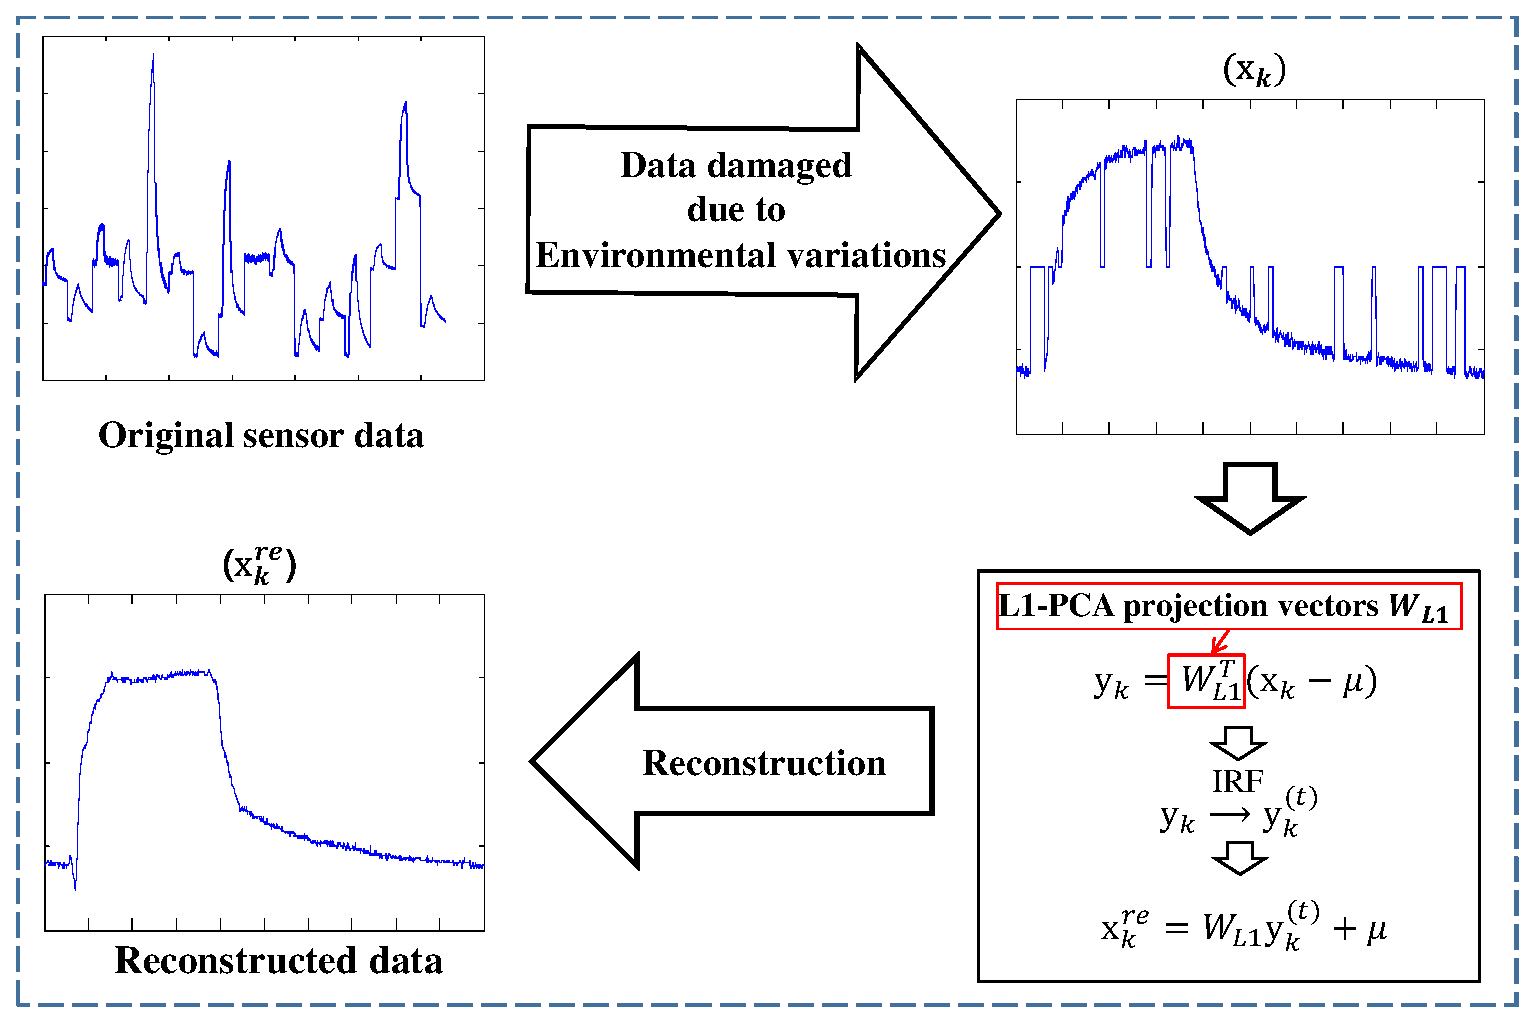
\includegraphics[width=0.8\textwidth]{_4.eps}
    \caption{\bf{Overall procedure of the proposed data reconstruction method.}\label{Fig. 4}}
\end{figure}

In order to determine the optimal \textit{m} value for data reconstruction, the root mean squared (RMS) error between the data before loss and the reconstructed data  defined as in \ref{eq:sic12} was calculated. 

\begin{eqnarray}
\label{eq:sic12}
	\mathrm E_{RMS} = \frac{1}{N}\sum\limits_{k=1}^{N}||\mathbf{x}_k-\mathbf{x}_k^{re}||_2
\end{eqnarray}


Fig. \ref{Fig. 3} shows the RMS errors when the data is reconstructed using the $W_{L1}$ composed of \textit{m} L1-PCA projection vectors and the feature vector $\textbf{y}^{(t)}$ while varying the value of \textit{m}, given a loss of an arbitrary ratio to the values of the training data samples. 
In Fig. \ref{Fig. 3}, it can be seen that the optimal $m$ differs depending on the degree of data loss. 

This shows that as the loss ratio increases, it is more effective to use a smaller number of projection vectors for reconstruction. 
This means that if the loss of data is large, it is more effective to not use the features extracted by the projection vector with a small eigenvalue, which are susceptible to noise, in reconstructing the data.
In this paper, experiments on training data were performed to determine the $m$ value showing the minimum RMS error for the reconstruction process according to the loss ratio.



Fig. \ref{Fig. 4} shows the overall procedure of the proposed data reconstruction method using the iterative reweighted L1-PCA. 

\begin{figure}[h]
	\centering
    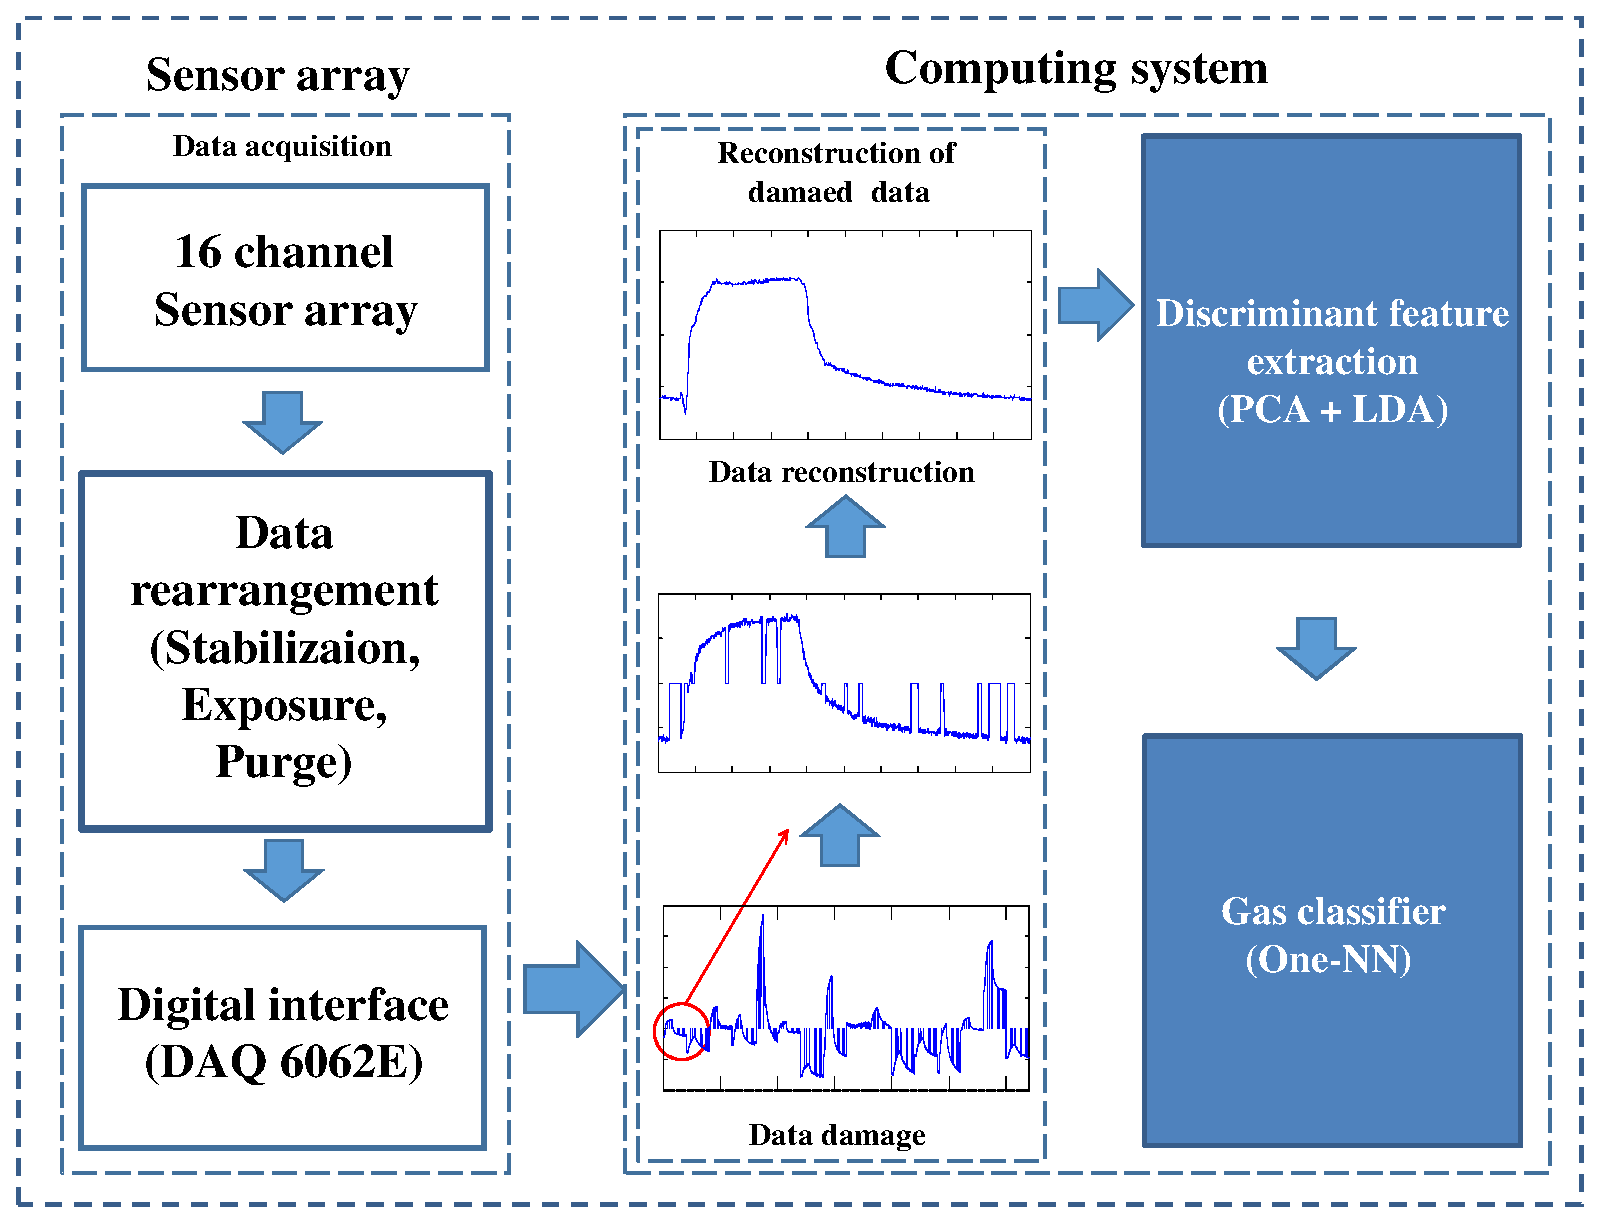
\includegraphics[width=0.8\textwidth]{_5.eps}
    \caption{\bf{Schemetic diagram of our electronic nose system.}\label{Fig. 5}}
\end{figure}


\begin{table}[h]
\centering
\caption{CB polymer composites in the sensor array.}
\label{table1}
\begin{tabular}{|c|c|}
\hline
Channel & Polymer                                               \\ \hline
1       & Poly(methyl methacrylate)                             \\ \hline
2       & Polyvinylpyrrolidone                                  \\ \hline
3       & Poly(vinyl acetate)                                   \\ \hline
4       & Poly(ethylene oxide)                                  \\ \hline
5       & Polycaprolactone                                      \\ \hline
6       & Poly(4-methylstyrene)                                 \\ \hline
7       & Poly(styrene-co-methyl methacrylate)                  \\ \hline
8       & Poly(enthylene-co-vinylacetate)                       \\ \hline
9       & Poly(bisphenol A carbonate)                           \\ \hline
10      & Poly(4-vinyl pyridine)                                \\ \hline
11      & Poly(vinyl butyral)-co-vinyl alcohol-co-vinyl acetate \\ \hline
12      & Poly(vinyl stearate)                                  \\ \hline
13      & Ethyl cellulose                                       \\ \hline
14      & Polystyrene-block-polyisoprene-block-polystyrene      \\ \hline
15      & Hydroxypropyl cellulose                               \\ \hline
16      & Cellulose acetate                                     \\ \hline
\end{tabular}
\end{table}

\section*{Design of Electronic Nose System}
\subsection*{Data Acquisition}
\begin{figure}[t]
	\centering
    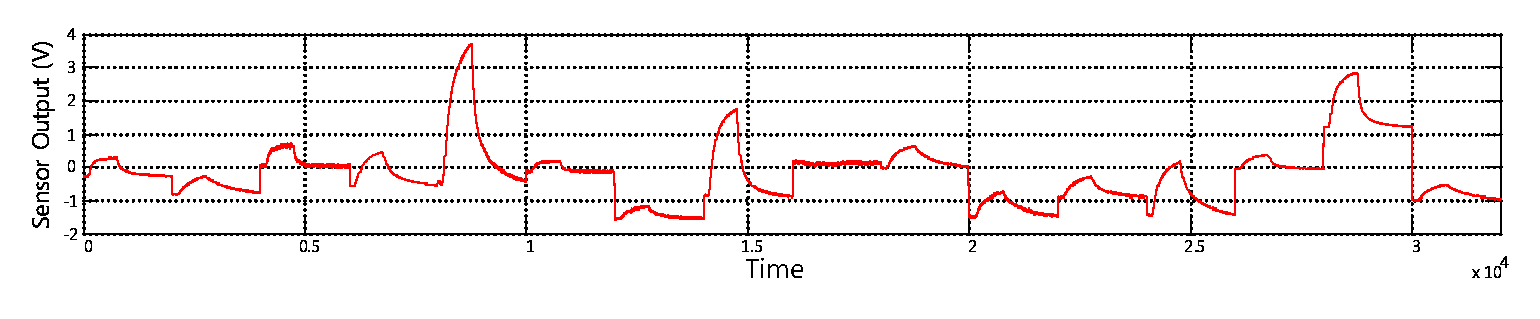
\includegraphics[width=1\textwidth]{_6.eps}
    \caption{\bf{Representation of data sample in 32,000 dimensional vector form.}\label{Fig. 6}}
\end{figure}

Fig. \ref{Fig. 5} shows a schematic diagram of the electronic nose system used in this paper.
While polymer composites have limitations in sensor life, sensor drift, and sensitivity to temperature and humidity, they are widely used in electronic nose systems compared to other gas sensors due to low cost, low power, stable operation at room temperature, etc. \cite{choi2014discriminant,wang2007reconstruction,vergara2012chemical}. 

In the electronic nose system used in this paper, a micoromachined sensor array chip used in \cite{wang2007reconstruction} was used. 
The sensor array consists of 16 channels, and each channel has a carbon-black (CB) polymer composites sensor with an interdigitated electrode, a microheater, and a machined membrane. Table \ref{table1} shows 16 types of (CB) polymer composites. 
The measurement of the sensor was performed by observing the change in resistance when the chemical gas was bonded to each polymer composite film and recording it for a total of 200 seconds at 0.1 second intervals.

First, after the sensor array is placed in the chamber and the resistance signal stabilizes for 30 seconds (stabilization), the flow control of the system exposes the gas for 60 seconds (exposure) and leaves the remaining gas to the outside for 110 seconds\cite{ha2005integrated}. The measured data are stored on a PC using the DAQ6062E data acquisition (DAQ) board and LabVIEW (National Instrumentation, USA). The voltage-divider operates from -10V to 10V and the gain of 16 identical amplifiers is set to 10 for maximum DAQ resolution\cite{yang2005matched}.

\subsection*{Feature Extraction for Classification from Reconstructed Data}

If extracting features that are effective for gas classification from the reconstructed data, the classifier takes these features as inputs and finally determines the type of gas. 
In this paper, we use the linear discriminant analysis (LDA) method \cite{fukunaga2013introduction}, which is a typical supervised learning method, as a feature extraction method for classification. 
LDA constructs a low-dimensional feature space such that the ratio of the variance of each class mean and the variance of the samples in the same class increases. Feature extraction methods other than LDA can also be employed for this purpose; LDA was selected in this study for convenience.

When $N$ training data samples $\textbf{x}_k$ $(k=1,...,N)$ are composed of $C$ classes and each class $c_i$ $(i=1,...,C)$ has $N_i$ samples, the between-class scatter matrix ($S_{B}$) and the within-class scatter matrix ($S_{W}$) are defined as follows.

\begin{figure}[t]
	\centering
    \includegraphics[width=1\textwidth]{_7.eps}
    \caption{\bf{Representation of the lost data sample and reconstructed data sample. (a) $\textbf{x}_{10\%}^{dmg}$ (b) $\textbf{x}_{10\%}^{re}$}\label{fig. 7}}
\end{figure}

\begin{figure}[t]
	\centering
    \includegraphics[width=1\textwidth]{_8.eps}
    \caption{\bf{Representation of the lost data sample and reconstructed data sample. (a) $\textbf{x}_{20\%}^{dmg}$ (b) $\textbf{x}_{20\%}^{re}$}\label{fig. 8}}
\end{figure}

\begin{gather}
\label{eq:sic13}
	\mathrm S_B = \frac{1}{N}\sum\limits_{i=1}^{C}N_i(\mu_i-\mu)(\mu_i-\mu)^T \nonumber\\
    S_W = \sum\limits_{i=1}^{C}\sum\limits_{\mathbf{x}_k\in{c}_{i}}^{ }(\mathbf{x}_k-\mu_i)(\mathbf{x}_k-\mu_i)^T \nonumber \\
    \mu_i = \frac{1}{N_i}\sum\limits_{{\mathbf{x}_k}\in{c_i}}^{}\mathbf{x}_k,\quad \mu = \frac{1}{N}\sum\limits_{i=1}^{C}\sum\limits_{{\mathbf{x}_k}\in{c_i}}^{}\mathbf{x}_k
\end{gather}

LDA constitutes a feature space that can be distinguished between classes by maximizing the ratio of $S_B$ and $S_W$. Therefore, the objective function of LDA can be expressed as follows. 


\begin{eqnarray}
\label{eq:sic14}
	\mathrm W_{LDA} = \textrm{arg} \underset{W}{\textrm{max}}\frac{|W^{T}S_{B}W|}{|W^{T}S_{W}W|}
\end{eqnarray}

The solution satisfying (\ref{eq:sic14}) corresponds to the eigenvector of $S_W^{-1}S_B$. 
In the high-dimensional data such as the electronic nose sensor data, the small sample size (SSS) problem \cite{chen2000new} occurs in which the number of training data is smaller than the dimension of training data, and no inverse matrix is available. 
To avoid this problem, we first reduce the dimension of data to less than the rank of $S_W$ using PCA and then applied LDA in the PCA feature space (PCA + LDA \cite{belhumeur1997eigenfaces}). If letting the projection matrix of the PCA be $W_{PCA}$, the final projection matrix by PCA + LDA can be expressed as follows.


\begin{eqnarray}
\label{eq:sic15}
	\mathrm W_{PCA+LDA} = W_{LDA}^{T}W_{PCA}^{T}\nonumber\\\nonumber\\W_{LDA} = \textrm{arg} \underset{W}{\textrm{max}}\frac{|W^{T}W_{PCA}^{T}S_{B}W_{PCA}W|}{|W^{T}W_{PCA}^{T}S_{W}W_{PCA}W|}
\end{eqnarray}


If selecting $n' (\le C-1)$ projection vectors constituting $W_{PCA+LDA}$ in order of their eigenvalues, the gas data sample $\textbf{x}_k$ is an $n'$-dimensional feature vector composed of $n'$ discriminant features as follows.

\begin{figure}[t]
	\centering
    \includegraphics[width=1\textwidth]{_9.eps}
    \caption{\bf{Representation of the lost data sample and reconstructed data sample. (a) $\textbf{x}_{30\%}^{dmg}$ (b) $\textbf{x}_{30\%}^{re}$}\label{fig. 9}}
\end{figure}

\begin{figure}[t]
	\centering
    \includegraphics[width=1\textwidth]{_10.eps}
    \caption{\bf{Representation of the lost data sample and reconstructed data sample. (a) $\textbf{x}_{40\%}^{dmg}$ (b) $\textbf{x}_{40\%}^{re}$}\label{fig. 10}}
\end{figure}


\begin{eqnarray}
\label{eq:sic16}
	\mathbf{y}_\mathrm{k}^L = W_{PCA+LDA}^T(\mathbf{x}_k-\mu)=[y_{k1}^{L},y_{k2}^{L},..,y_{kn'}^{L}]^T
\end{eqnarray}


\section*{Experimental Results}

In order to verify the effectiveness of the proposed method, we attempted to classify the volatile organic compounds (VOCs) measurement data for 8 types of gases. 
The gases used in the experiments were acetone, benzene, cyclo-hexane, ethanol, heptane, methanol, propanol, and toluene \cite{yang2005matched}. Twenty samples were collected for each type of gas and a total of 160 samples were collected. Each sample consists of the measurements for 2,000 time points measured at a sampling rate of 10 Hz per channel for 200 seconds. 
The measurement values of 16 channels are stored in the form of 2,000$\times$16 matrix, and then converted to a 32,000 dimensional vector using a lexicographic ordering operator \cite{choi2014discriminant} (Fig. \ref{Fig. 6}).

To see the effectiveness of the proposed method in reconstructing the data, we analyzed the performance for the data samples with data loss of 10\% ($\textbf{x}_{10\%}^{dmg}$), 20\% ($\textbf{x}_{20\%}^{dmg}$), 30\% ($\textbf{x}_{30\%}^{dmg}$), and 40\% ($\textbf{x}_{40\%}^{dmg}$) of the total measurements. 
For this purpose, considering the electrical problems that may occur in the actual electronic nose installation environment, it is assumed that the loss interval occurs in 2 second units (20 time points), and the data value of the corresponding interval is set to zero. 
All data values used in the experiments were normalized \cite{choi2014discriminant} using the mean and standard deviation of the training data. 
The optimal value of $m$ for each loss ratio was set to a value representing the minimum RMS for the training data.

Figs. \ref{fig. 7}-\ref{fig. 10} show (a) the data samples having the loss ($\textbf{x}^{dmg}$) and (b) the reconstructed samples($\textbf{x}^{re}$). 
In (b) of each figure, the red line shows the original data (no loss) and the blue line shows the reconstructed data. 
Although the error between the original data and the reconstructed data increases as the loss ratio increases, it is confirmed that the shapes of the lost data samples were reconstructed similarly to the respective shapes of the original data. 


For a total of 160 gas data samples of 8 types, the gas classification experiments were conducted to verify the effect of the data reconstruction on the gas classification performance of the electronic nose. 
All samples were tested using 8-fold cross validation \cite{liu2009encyclopedia}. 
In other words, data were randomly mixed and then divided into training data sets consisting of 140 samples and test data of 20 samples for each fold. The final classification rates were calculated by averaging the classification rates in 8 experiments. 

As mentioned previously, the discriminant features to be used as input to the classifier were extracted using the PCA + LDA method.
In the PCA phase of PCA+LDA, the dimension of original sample space (32,000 dim.) was reduced to the 105 dimensional feature space corresponding to 99\% of the total eigenvalues of $S_T$, and then, LDA was performed in the reduced feature space. 
Since the PCA+LDA method can extract up to 7 features in the problem of 8 classes, the classification performance is measured in the 7-dimensional PCA + LDA feature space. 
One-nearest neighbor (One-NN) classifier was used as the classifier, and the distance between samples was measured based on L2-norm \cite{wang2007reconstruction}.

\begin{figure}[t]
	\centering
    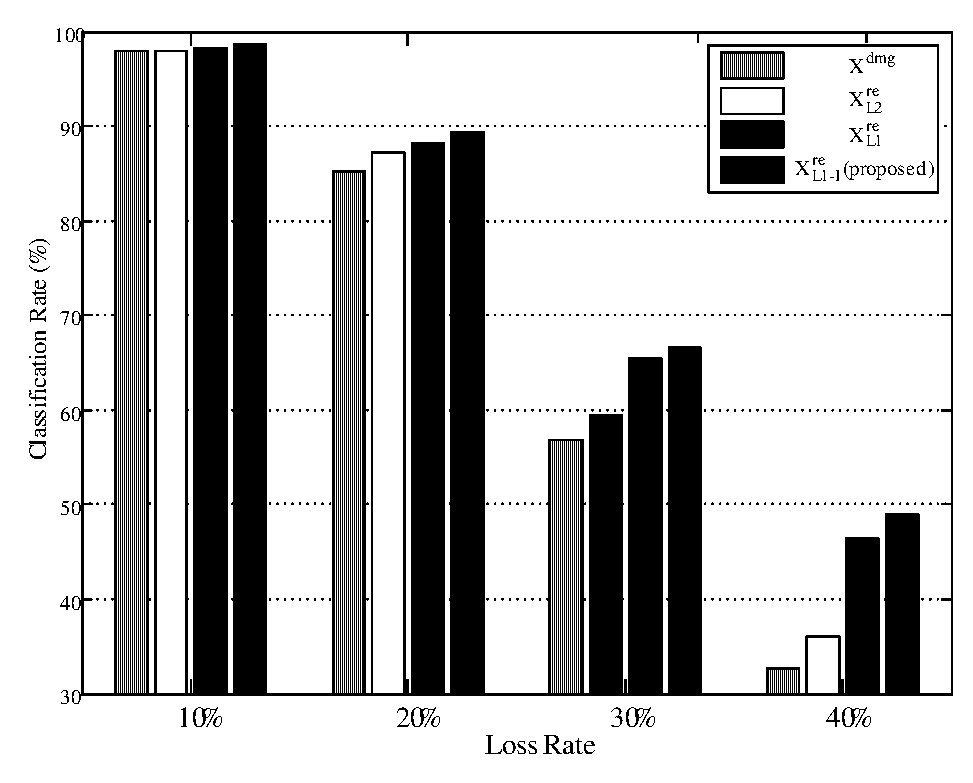
\includegraphics[width=0.8\textwidth]{_11.eps}
    \caption{\bf{Compression of classification rates between the proposed method and other methods}\label{fig. 11}}
\end{figure}

Fig. \ref{fig. 11} shows the classification rates for the loss data $(\textbf{x}^{dmg})$, the reconstructed data using L2-PCA $(\textbf{x}^{re}_{L2})$, the reconstructed data using L1-PCA $(\textbf{x}^{re}_{L1})$, and the proposed method $(\textbf{x}^{re}_{L1-I})$ for the data loss rates of 10\%, 20\%, 30\%, and 40\%. 
As shown in Fig. \ref{fig. 11}, $\textbf{x}^{re}_{L2}$, $\textbf{x}^{re}_{L1}$, and $\textbf{x}^{re}_{L1-I}$ show good data reconstruction performance when the amount of data loss is small (10\%). 
Even when the data was not reconstructed, the classification rate was as high as 97.89\%, which indicates that the features of the PCA + LDA itself are fairly robust when the data damage is small. 
However, as the amount of data loss increased from 20\% to 30\% and 40\%, the classification rates decreased significantly in the absence of data reconstruction. 
This is because the data samples that were more than 20\% lost seem to have lost much of the inherent characteristics of the class in the PCA + LDA feature space. 
On the other hand, in the case of the data reconstruction process, even if 20\% data loss occurred, the classification performance of 85\% or more could be maintained, and the experiments on 30\% and 40\% data loss show that the classification rates of data reconstructed by the proposed method were the highest.

\section*{Conclusions}
In an electronic nose system, data loss caused by the installation environment or electrical instability of the sensor deteriorates the stability of the gas classification performance. In this paper, we proposed a method to reconstruct the damaged data effectively to improve the stability of the electronic nose system. PCA is used not only for dimension reduction or representation of high-dimensional data such as electronic sensor data, but also for reconstructing the original dimension data by a linear combination of projection vectors and the PCA features. 
We used L1-norm based PCA, instead of conventional L2-norm based PCA, to reduce the influence of outlier data. 
In addition, by repeatedly updating the features using the generalized objective function for the reconstruction error, we reduced the distortion of the L1-PCA features due to the outlier samples, and obtained high-quality features. 
The damaged data samples were reconstructed by the weighted linear combination of the projection vectors of L1-PCA and the updated features.  

In order to verify the effectiveness of the proposed method, the reconstruction and gas classification experiments were performed with eight types of gas data measured by the carbon-black sensor.
As a result, the lost data was reconstructed to a shape similar to the original data. 
The result of the gas classification experiment on the reconstructed data confirmed that the data reconstruction process mitigates the deterioration of the gas classification performance due to the data loss. 

In the future, experiments will be conducted on more diverse types of complex data, and research will be performed combining various types of features effectively.

\section*{Acknowledgments}
This research was supported by the MSIT(Ministry of Science and ICT), Korea, under the ITRC(Information Technology Research Center) support program (IITP-2015-0-00363) and the National Program for Excellence in SW (IITP-2017-0-00091)
supervised by the IITP(Institute for Information and communications Technology Promotion)“

\section*{Author Contributions}
Conceived and designed the experiments: HJ SC. Performed the experiments: HJ. Analyzed
the data: HJ SC. Contributed reagents/materials/analysis tools: HJ. Wrote the paper: HJ JL GJ SC
ML. Discussed idea in this paper: HJ JL GJ SC.

\bibliography{electronic_nose}
\end{document}

